\begin{figure*}[tb]
	\begin{minipage}[b]{.8\textwidth}
		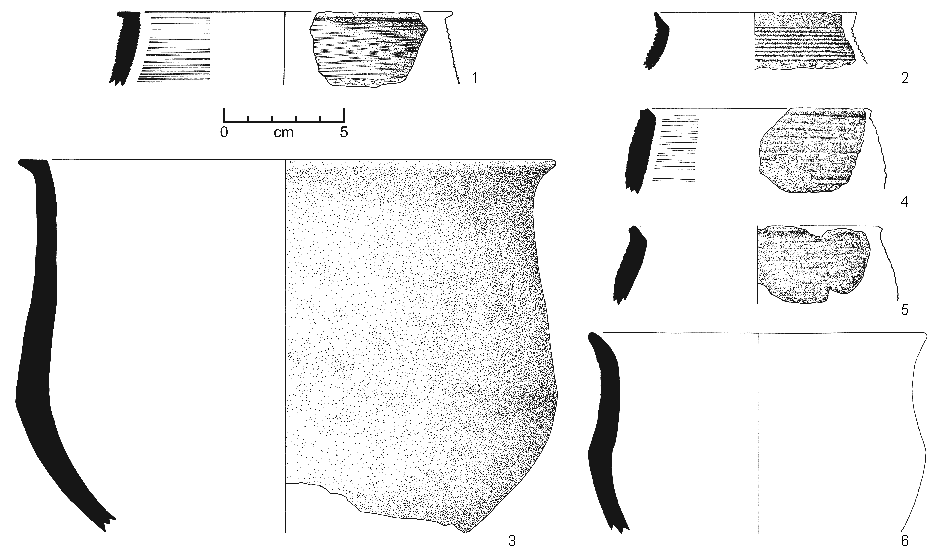
\includegraphics[width=.95\textwidth]{fig/MAT-Typen.pdf}
	\end{minipage}\hfill
	\begin{minipage}[b]{.2\textwidth}
		\caption{Matoto-Gruppe: Typvertreter.\\1:~Taf.~59.26; 2:~Taf.~59.1; 3:~Taf.~87.3; 4:~Taf.~59.30; 5:~Taf.~59.29; 6:~Taf.~21.2.}
		\label{fig:MAT_Typvertreter}
	\end{minipage}
\end{figure*}

\subsubsection{Matoto-Gruppe}\label{sec:MAT-Gr}

Die Matoto-Gruppe beschreibt eine nahezu im gesamten Arbeitsgebiet angetroffene Keramik, welche sich vor allem durch ihre charakteristischen Gefäßmorphologie auszeichnet. Dabei handelt es sich konkret um Gefäße mit gerader Wandung und sehr kurzen, teilweise scharf umbiegenden Rändern (Abb.~\ref{fig:MAT_Typvertreter}). Insgesamt konnten 60 GE dieser Stilgruppe zugeordnet werden, während 15 weitere GE nur unter Vorbehalt der Matoto-Gruppe zuzurechnen sind. Überdies wurden weitere 33 Randscherben aus Mandombe (Fpl.~259) und Motoli (Fpl.~261) am \mbox{Sangha}, die sämtlich sicher der Matoto-Gruppe zuordnet werden konnten, summarisch erfasst. Die Matoto-Gruppe setzt sich fast ausschließlich aus Randstücken zusammen (95\,\%). Lediglich ein hinreichend vollständiges Gefäß (Abb.~\ref{fig:MAT_Typvertreter}.3) konnte dieser Stilgruppe zugewiesen werden. Während ein großer Teil des keramischen Materials der Matoto-Gruppe aus Mandombe am mittleren \mbox{Sangha} (Fpl.~259) stammt, insgesamt wurden hier 31~GE und 30 ausgezählte Randstücke der Matoto-Gruppe nachgewiesen, wurden an insgesamt 17 weiteren Fundorten entlang der Flussläufe des \mbox{Sangha}, \mbox{Likwala}-\mbox{aux}-\mbox{Herbes} und \mbox{Ubangi} sowie am Lua immer wieder vereinzelte GE der Matoto-Gruppe (\textless\,9~GE) bei Surveys entdeckt. Mit Blick auf die individuell aufgenommenen GE macht das Inventar aus Mandombe 41\,\% aller der Matoto-Gruppe zugerechneten Stücke aus.\footnote{Da die Fundstelle Mandombe (Fpl.~259) bereits als eponymer Name für eine andere keramische Stilgruppe herangezogen wurde (Kap.~\ref{sec:MDB-Gr}), wurde die mit neun GE zwar eindeutig ärmere, jedoch auch das zweitgrößte Fundinventar aufweisende Fundstelle Matoto am mittleren \mbox{Sangha} (Fpl.~264) als eponyme Fundstelle für die Stilgruppe ausgewählt. Matoto liegt nur etwa 20\,km stromauf beziehungsweise nördlich von Ma"-ndo"-mbe und fällt in das Hauptverbreitungsgebiet der Stilgruppe.} Etwa 87\,\% aller Stücke stammen aus Absammlungen von Oberflächen. Die Funde aus Mandombe wurden vornehmlich zwischen aufgelassenen, alten Hausstellen gemacht. Acht GE der Matoto-Gruppe wurden oberhalb der Grube MLB~85/1-3-1 (Kat.-Nr.~1) in Maluba am Lua (Fpl.~230) erfasst.\footnote{Im ersten Abtrag fanden sich sechs GE und in den Abträgen 3 sowie 4 jeweils ein weiteres Randstück, das der Matoto-Gruppe zugerechnet werden kann.} Zwei weitere GE der Matoto-Gruppe wurden im zweiten und dritten Abtrag der Grabung PIK~87/1 gefunden (Kat.-Nr.~8; Taf.~48.11).


\paragraph{Technologische Merkmale}\hspace{-.5em}|\hspace{.5em}%
Die Scherben der Matoto-Gruppe zeigen eine starke Heterogenität der \textit{Fabrics}. Fast dreiviertel aller Scherben weisen hohe (54\,\%) bis sehr hohe (20\,\%) Anteile nichtplastischer Partikel auf. Diese sind größtenteils den Größenklassen \textit{medium} (32\,\%) sowie \textit{coarse} (46\,\%) zuzurechnen. Es handelt sich fast ausschließlich um Quarzsande (84\,\%). Selten enthalten die Scherben auch ausgebrannte Organik sowie Glimmer oder Laterit. In Bezug auf die Färbung der Scherben weisen über die Hälfte aller Stücke (51\,\%) auf die Nutzung weißbrennender Tone hin, während jeweils etwa ein Viertel der Stücke rotbrennende Tone andeuten (25\,\%) oder keine Aussagen zulassen (24\,\%). Nur 26\,\% der Scherben zeigen geglättete Oberflächen, während 53\,\% leicht raue und 18\,\% deutlich raue Oberflächen aufweisen. Die GE der Matoto-Gruppe zeigen eine mittlere Wandungsdicke von 6,2\,mm.

\begin{figure*}[p]
	\centering
	\includegraphics[width=\textwidth]{fig/MAT_Verbreitung.pdf}
	\caption{Matoto-Gruppe: Verbreitung.}
	\label{fig:MAT_Verbreitung}
\end{figure*}

\paragraph{Formen}\hspace{-.5em}|\hspace{.5em}%
Lediglich bei zwei GE der Matoto-Gruppe konnte die Gefäßform sicher angesprochen werden, während bei acht weiteren GE eine Ansprache der Gefäßform unter Vorbehalt vorgenommen werden konnte. Die beiden sicher angesprochenen Stücke zeigen ein gerades beziehungsweise nur leicht konkaves Oberteil, einen leichten Bauchknick sowie ein konvexes Unterteil und sind der Gefäßform F1 zuzurechnen. Sie stammen vom Likwala-aux-Herbes, Flusskilometer~401 (Fpl.~301; Abb.~\ref{fig:MAT_Typvertreter}.3) sowie aus Mboko~I am \mbox{Ubangi} (Fpl.~217; Abb.~\ref{fig:MAT_Typvertreter}.6). Obschon viele der Randstücke zu einer sehr ähnlichen Gefäßform gehört haben könnten (Abb.~\ref{fig:MAT_Typvertreter}.1--2, 4--5), lässt sich aufgrund mangelnder Erhaltung der Gefäßprofile keine belastbare Aussage treffen. Der maximale Durchmesser der Gefäße schwankt zwischen 14--22\,cm, bei einer Mündungshöhe von 11,5--17\,cm.  Da nur wenige größere Scherben der Matoto-Gruppe vorhanden sind, liegen auch kaum Informationen über die Ausgestaltung der Gefäßbäuche vor. Lediglich bei fünf GE war der Gefäßbauch erhalten. Vier GE zeigen die typischen, leichten Bauchknicke, die für die Gefäßform F1 charakteristisch sind. Die bestimmenden Randformen der Matoto-Keramik sind kurz umgelegte (A2; 39\,\%; Abb.~\ref{fig:MAT_Typvertreter}.1, 3) sowie ausbiegende Ränder (B1; 44\,\%; Abb.~\ref{fig:MAT_Typvertreter}.2, 4--5). Die Mündungsabschlüsse der Ränder sind regelhaft spitz zulaufend (M2; 34\,\%) oder gerillt (M4; 33\,\%). Deutlich seltener fanden sich rund abgeschlossene (M1; 9\,\%) sowie schräg nach außen abgestrichene Mündungen (M5; 7\,\%). Der Halsbereich der Matoto-Gefäße ist häufig leicht kegelförmig bis zylindrisch. Nur sechs GE zeigen einen ausgeprägten Schulterbereich, welcher entweder gerade oder leicht konvex ist. Bei zwei GE, beide stammen aus Yumba am \mbox{Likwala}-\mbox{aux}-\mbox{Herbes} (Fpl.~289), ließ sich die Form des Gefäßbodens ermitteln. Beide Stücke weisen runde Böden auf (B1). Die Zuordnung beider Stücke zur Matoto-Gruppe ist jedoch nicht zweifelsfrei. Aus dem restlichen Fundmaterial sind keine Bodenscherben der Matoto-Gruppe bekannt, so dass keine belastbaren Aussagen über die Gestaltung der Böden der Matoto-Keramik gemacht werden können.

\paragraph{Verzierungen}\hspace{-.5em}|\hspace{.5em}%
Die Verzierungen der Matoto-Gruppe werden von horizontalen Rillen (Tab.~\ref{tab:Verzierungselemente}: 02.1) bestimmt, die 84\,\% aller Verzierungselemente ausmachen und sich fast ausschließlich und zu gleichen Teilen auf der Innenseite der Ränder sowie im Halsbereich finden (Abb.~\ref{fig:MAT_Typvertreter}.1--2,4; Anlage~4\subref{fig:MAT_Verz}). Insgesamt lassen sich 87\,\% aller beobachteten Verzierungselemente diesen beiden Gefäßzonen zuordnen. Unterhalb des Schulterbereichs ließen sich keine Verzierungen beobachten, was allerdings auch der Tatsache geschuldet ist, dass sich die Matoto-Gruppe fast ausschließlich aus Randscherben zusammensetzt und andere Gefäßzonen deutlich unterrepräsentiert sind. Neben den horizontalen Rillen finden sich nur sehr selten weitere Verzierungselemente. Unter anderem handelt es sich dabei um Reihen aus kleinen diagonalen oder vertikalen Ritzlinien (Tab.~\ref{tab:Verzierungselemente}: 04.15; 7\,\%), Reihen aus dreieckigen oder quadratischen Eindrücken (Tab.~\ref{tab:Verzierungselemente}: 04.12; 3\,\%) sowie runden Eindrücken (Tab.~\ref{tab:Verzierungselemente}: 04.11; 2\,\%) und diagonales Schachbrettmuster (Tab.~\ref{tab:Verzierungselemente}: 01.2; 1\,\%; Abb.~\ref{fig:MAT_Typvertreter}.4--5). Alle beobachteten Verzierungen sind grundsätzlich sehr fein ausgeführt.

\paragraph{Datierung}\hspace{-.5em}|\hspace{.5em}%
Für die Keramik der Matoto-Gruppe liegen keine direkten Datierungen vor. Lediglich im Fundgut, das der Bestattung in MLB~85/1-4-3 (Kat.-Nr.~3) in Maluba am Lua zugewiesen wurde, fanden sich neben Batalimo-Maluba-Keramik auch Stücke, die der Matoto-Gruppe zugerechnet werden können. Zwei Radiokohlenstoffdatierungen an Knochenmaterial datieren in das 11.--14.~Jh. n.~Chr. (Tab.~\ref{tab:MLB85_1-4-3_14C}). Da das mit der Bestattung assoziierte keramische Material jedoch nicht als dezidierte \textit{Beigabe} zu interpretieren ist (siehe Kat.-Nr.~3), kann dieser Datierungsansatz lediglich als \textit{terminus ante quem} herangezogen werden; die Matoto-Gruppe muss also im 11.--14.~Jh. n.~Chr. bereits bestanden haben.

Stilistische Vergleiche zu anderen Stilgruppen des Arbeitsgebietes ergeben sich nur zu den Gruppen Dongo (Kap.~\ref{sec:DON-Gr}) sowie Konda (Kap.~\ref{sec:KON-Gr}). Beide weisen, wie die Matoto-Keramik, im Randbereich eine Verzierung aus feinen Rillen auf. Die Keramik der Dongo-Gruppe weist, ähnlich der Matoto-Keramik, auch eher kurze, gerade ausbiegende Ränder sowie Grundformen mit teilweise eher schwach geschweiften Wandungen auf. Keine der als Vergleich heranzuziehenden Stilgruppen ist jedoch sicher im Chronologieschema (Abb.~\ref{fig:Chronologiesystem}) zu verankern, wodurch auch die genannten Bezüge zur Matoto-Gruppe starken Vorbehalten unterliegen.

Vor dem gegenwärtigen Quellenstand kann keine sichere chronologische Ansprache der Matoto-Keramik erfolgen. Einzig die Beobachtung entsprechender Stücke in der Verfüllung des Grabes MLB~85/1-4-3 in Maluba (Kat.-Nr.~3) zeigt an, dass die Stilgruppe zu diesem Zeitpunkt bereits bestanden haben muss. Vorläufig wird sie daher an den Beginn der Jüngeren Eisenzeit im Arbeitsgebiet beziehungsweise in das 11.--14.~Jh. n.~Chr. datiert.

\paragraph{Verbreitung}\hspace{-.5em}|\hspace{.5em}%
Die Keramik der Matoto-Gruppe ist nahezu über das gesamte Arbeitsgebiet verbreitet (Abb.~\ref{fig:MAT_Verbreitung}). Den nördlichsten Verbreitungspunkt bildet dabei Mboko~I am oberen \mbox{Ubangi} (Fpl.~217). Das Kerngebiet ist jedoch eine kleine Region am mittleren \mbox{Sangha} nördlich von Pikunda, zwischen Molanda (Fpl.~258) und der namensgebenden Fundstelle Matoto (Fpl.~264). Aus diesem Bereich stammen 88\,\% aller sicher der Matoto-Gruppe zugewiesenen GE. Am \mbox{Likwala}-\mbox{aux}-\mbox{Herbes} fand sich bei Flusskilometer 401 (Fpl.~301) im Uferbereich eines stark mit Termiten-Hügeln durchzogenen Gebietes ein unverziertes Gefäß des Matoto-Stils (Abb.~\ref{fig:MAT_Typvertreter}.3).